\documentclass[a4paper, 12pt]{article}

\usepackage{tikz}
\usetikzlibrary{automata}

\title{Autómata}
\begin{document}
\maketitle

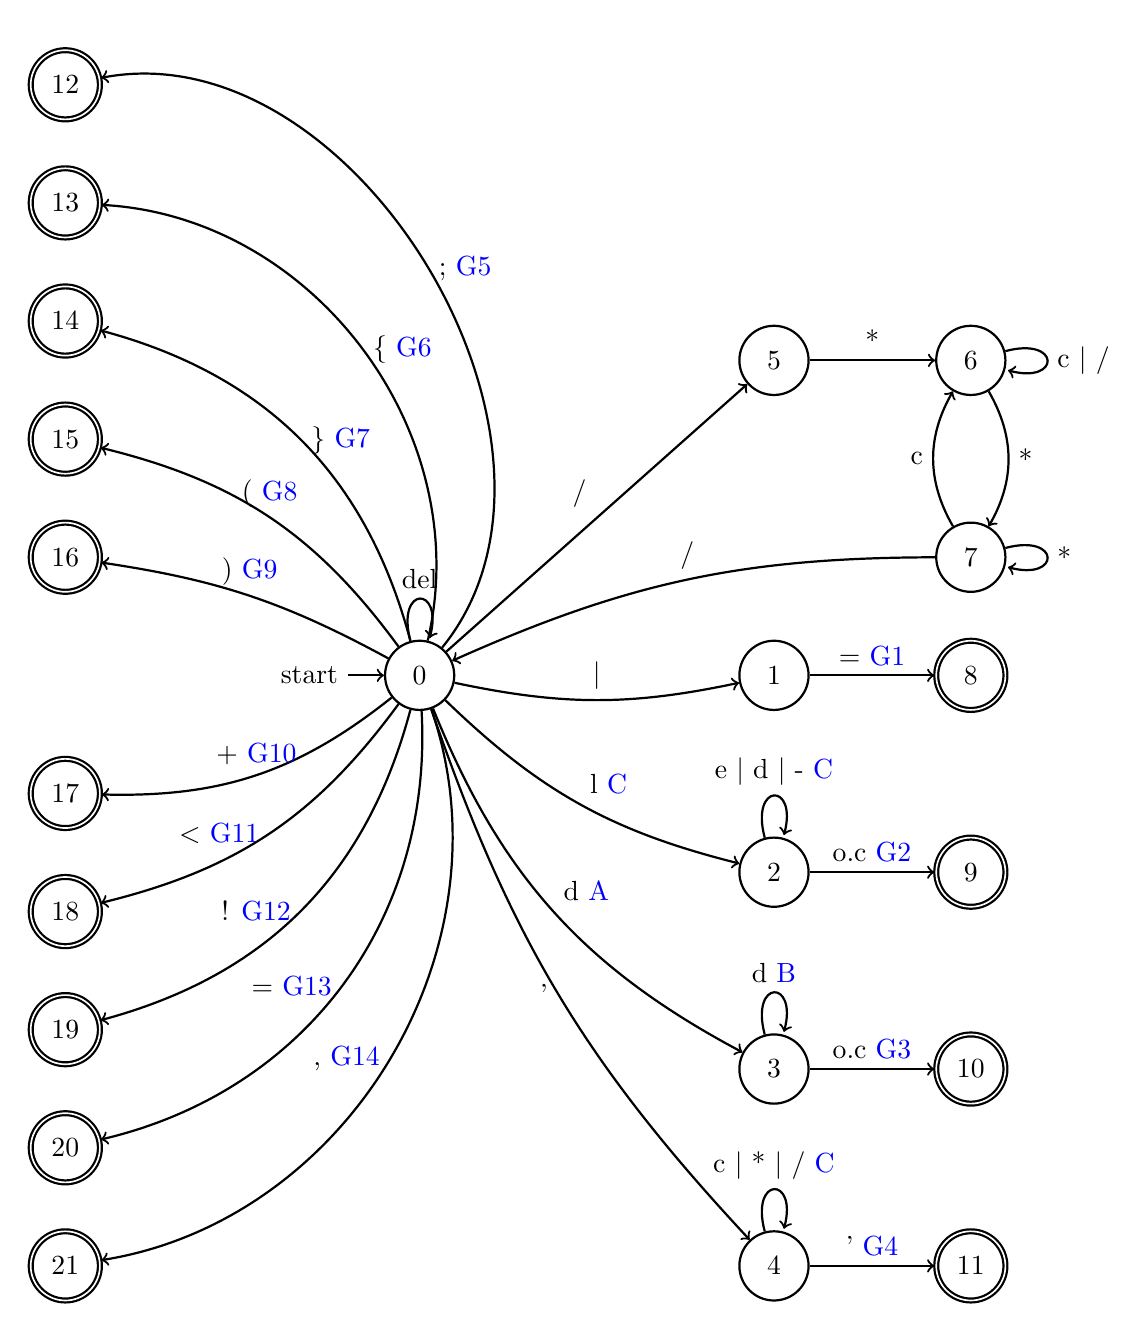
\begin{tikzpicture}[->,thick, node distance= 2.5cm,auto]
\tikzstyle{nodoChiquito} = [state, accepting, node distance = 1.5cm];
\node [state, initial](0){$0$};

\node [state](1)[right of = 0, xshift=2cm]{$1$};
\node [state, accepting](8)[right of = 1]{$8$};

\node [state](5)[above of = 1,yshift=1.5cm]{$5$};
\node [state](6)[right of = 5]{$6$};
\node [state](7)[below of = 6]{$7$};

\node [state](2)[below of = 1]{$2$};
\node [state, accepting](9)[right of = 2]{$9$};

\node [state](3)[below of = 2,]{$3$};
\node [state, accepting](10)[right of = 3]{$10$};

\node [state](4)[below of = 3]{$4$};
\node [state, accepting](11)[right of = 4]{$11$};

\node [nodoChiquito](12)[left of = 0,yshift=7.5cm,xshift=-3cm]{$12$};
\node [nodoChiquito](13)[below of = 12]{$13$};
\node [nodoChiquito](14)[below of = 13]{$14$};
\node [nodoChiquito](15)[below of = 14]{$15$};
\node [nodoChiquito](16)[below of = 15]{$16$};
\node [nodoChiquito](17)[below of = 16,yshift=-1.5cm]{$17$};
\node [nodoChiquito](18)[below of = 17]{$18$};
\node [nodoChiquito](19)[below of = 18]{$19$};
\node [nodoChiquito](20)[below of = 19]{$20$};
\node [nodoChiquito](21)[below of = 20]{$21$};

\path 
	(0) edge[loop above] node{del} (0)
        edge[bend right=70, right] node{; {\color{blue} G5}} (12)
        edge[bend right=50, right] node{\{ {\color{blue} G6}} (13)
        edge[bend right=30, right] node{\} {\color{blue} G7}} (14)
        edge[bend right=20, above] node{( {\color{blue} G8}} (15)
        edge[bend right=10, above] node{) {\color{blue} G9}} (16)
        edge[bend left=20, above] node{+ {\color{blue} G10}} (17)
        edge[bend left=20, left] node{$<$ {\color{blue} G11}} (18)
        edge[bend left=30, left] node{! {\color{blue} G12}} (19)
        edge[bend left=40, left] node{= {\color{blue} G13}} (20)
        edge[bend left=50, left] node{, {\color{blue} G14}} (21)
            
	    
	(0) edge [bend right=12] node{$\vert$} (1)
	(1) edge node{= {\color{blue} G1}} (8)
	
	(0) edge[bend right = 15] node{l {\color{blue} C}} (2)
	(2) edge [loop above] node{e $\vert$ d $\vert$ - {\color{blue} C} } (2)
	    edge node{o.c {\color{blue} G2}} (9)
	
	(0) edge[bend right = 20] node{d {\color{blue} A}} (3)
	(3) edge[loop above] node{d {\color{blue} B}} (3)
	    edge node{o.c {\color{blue} G3}} (10)
	    
	(0) edge[bend right=12,left] node{'} (4)
	(4) edge[loop above] node{c $\vert$ * $\vert$ / {\color{blue} C}} (4)
	    edge node{' {\color{blue} G4}} (11)
	
	(0) edge node{/} (5)
	(5) edge node{*} (6)
	(6) edge [bend left] node{*} (7)
	    edge [loop right] node{c $\vert$ /} (6)
	(7) edge [bend left] node {c} (6)
	    edge [loop right] node{*} (7)
	    edge[bend right=12, above] node {/} (0)

;



\end{tikzpicture}
\end{document}